% !TEX root = ../main.tex

A jelen fejezet a megvalósított rendszer által kiszámított mobilitási metrikák statisztikai jellemzőit, a napi aktivitásmintázatokat és az anomáliadetekció eredményeit mutatja be. A bemutatott számadatok mind a tényleges DuckDB-adatbázisból és a Parquet-fájlokból lekérdezett értékek.

\subsection{Mobilitási metrikák eloszlása}

A \autoref{fig:impl01} ábra a négy fő metrika eloszlását ábrázolja a dataset1-en (normál viselkedés). A gyrációs sugár és a home--work távolság erősen jobbra aszimmetrikus: a medián értékek lényegesen alacsonyabbak az átlagnál, ami hosszú farkú eloszlásra utal --- összhangban a González et al.\ \cite{gonzalez2008understanding} által leírt vágott hatványfüggvény-modellel, amelyet a szerzők szintén CDR adatokon igazoltak.

\begin{figure}[H]
\centering
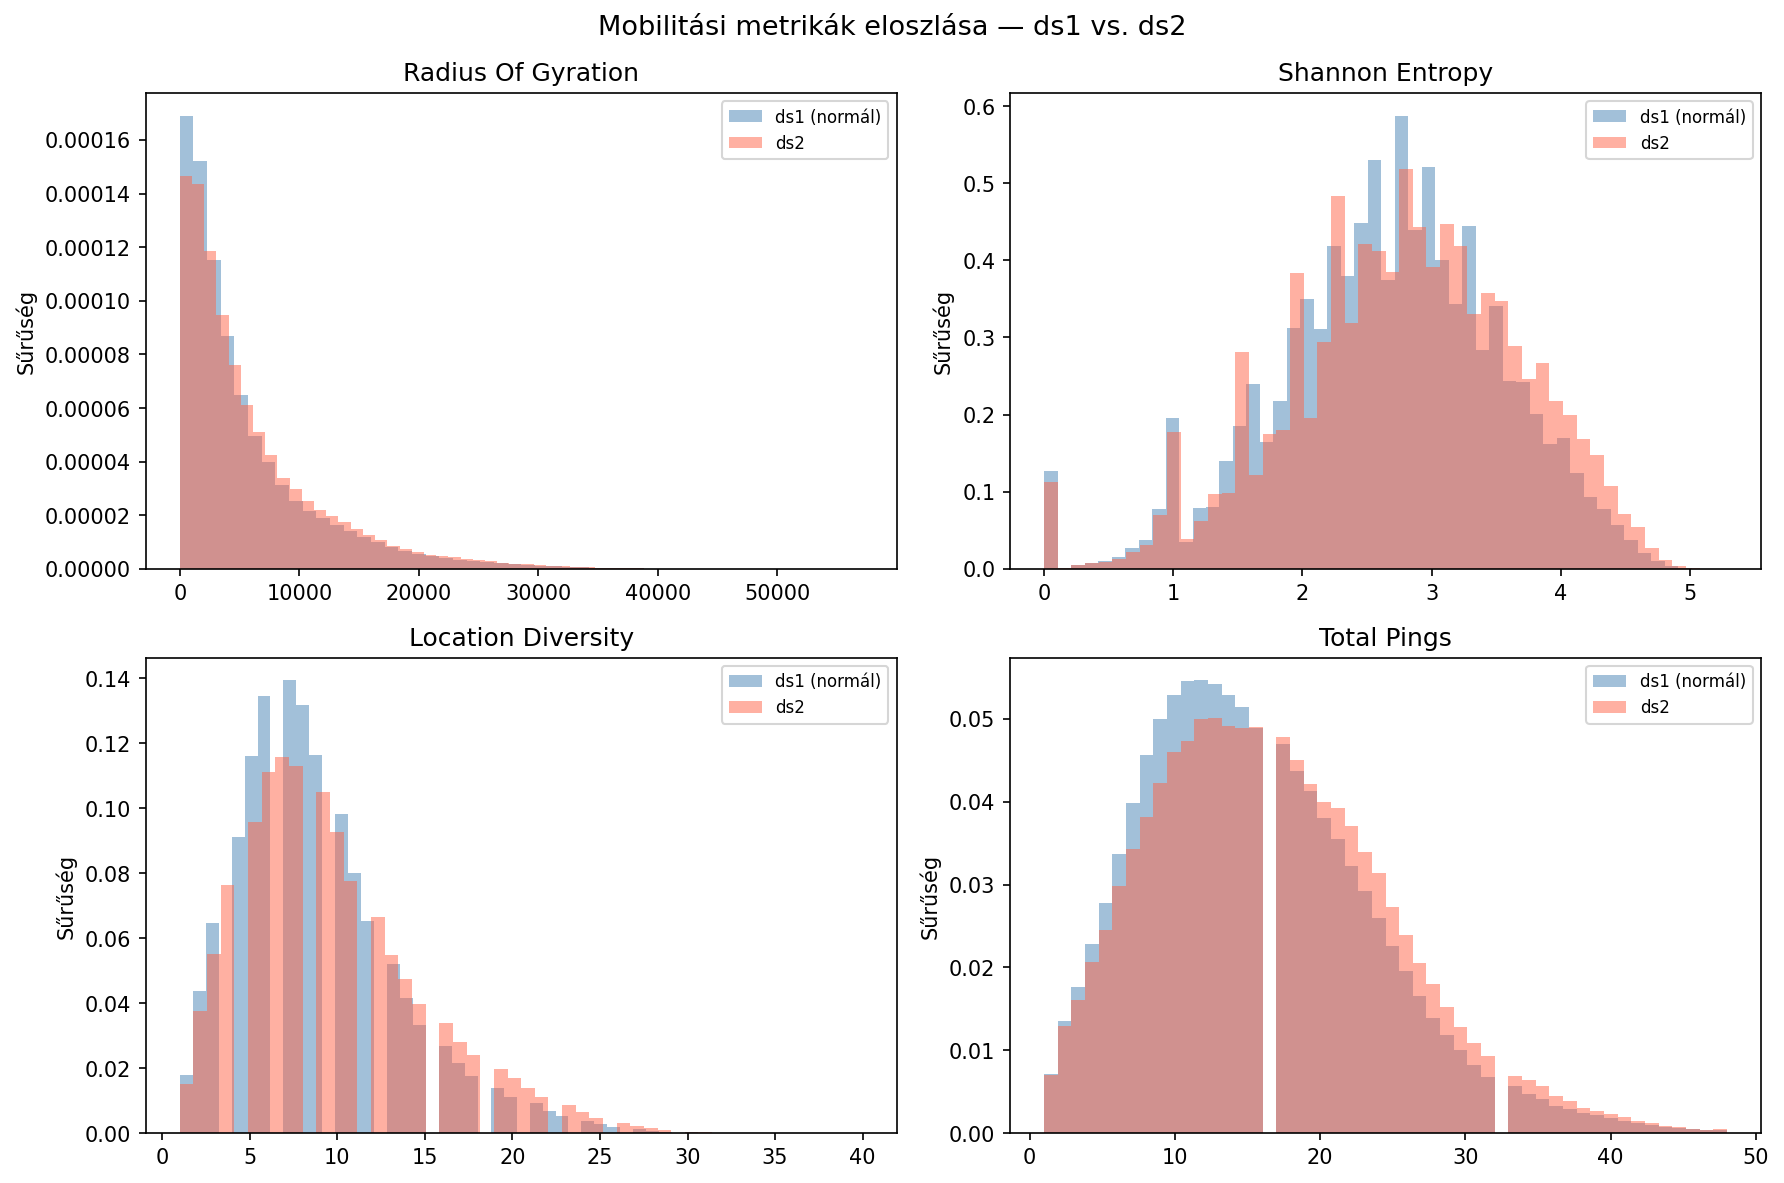
\includegraphics[width=0.95\textwidth]{img/impl_01_feature_distributions.png}
\caption{A négy mobilitási jellemző eloszlása a dataset1 normál időszakán. Saját számítás.}
\label{fig:impl01}
\end{figure}

Az alábbi táblázat (\autoref{tab:descriptives}) foglalja össze a kiszámított leíró statisztikákat:

\begin{table}[H]
\centering
\caption{A mobilitási jellemzők leíró statisztikái (dataset1, normál időszak).}
\label{tab:descriptives}
\begin{tabular}{l r r}
\hline
\textbf{Jellemző} & \textbf{Medián} & \textbf{Átlag} \\
\hline
Gyrációs sugár (m)           & 3~435  & 5~491  \\
Home--work távolság (m)      & 3~589  & 8~645  \\
Helydiverzitás (cella/nap)   & 8      & 8{,}84 \\
Shannon-entrópia (bit)       & --     & 2{,}66 \\
\hline
\end{tabular}
\end{table}

A felhasználók 27{,}8\%-a napi 10~km-nél nagyobb otthon--munkahely távolságot tesz meg --- ez az arány a japán nagyváros-környéki ingázási szokásoknak megfelelő értéket mutat. A jellemzők erősen jobbra aszimmetrikus, hósszan elnyúló farkat mutató eloszlása összhangban van González et al.\ \cite{gonzalez2008understanding} vágott hatványfüggvény-modelljével.

\subsection{POI-zónák aktivitása}

A \autoref{fig:impl02} ábra a cellánkénti aktivitás megoszlását mutatja POI-zóna és időszak szerint. A vészhelyzeti időszakban a szabadidős zónájú cellák aktivitása csökkent a legjobban, míg az ipari zónában szinte nem változott a mozgásszám --- összhangban azzal, hogy az ipari telephelyek üzemeltetése a korlátozások alatt is folytatódott.

\begin{figure}[H]
\centering
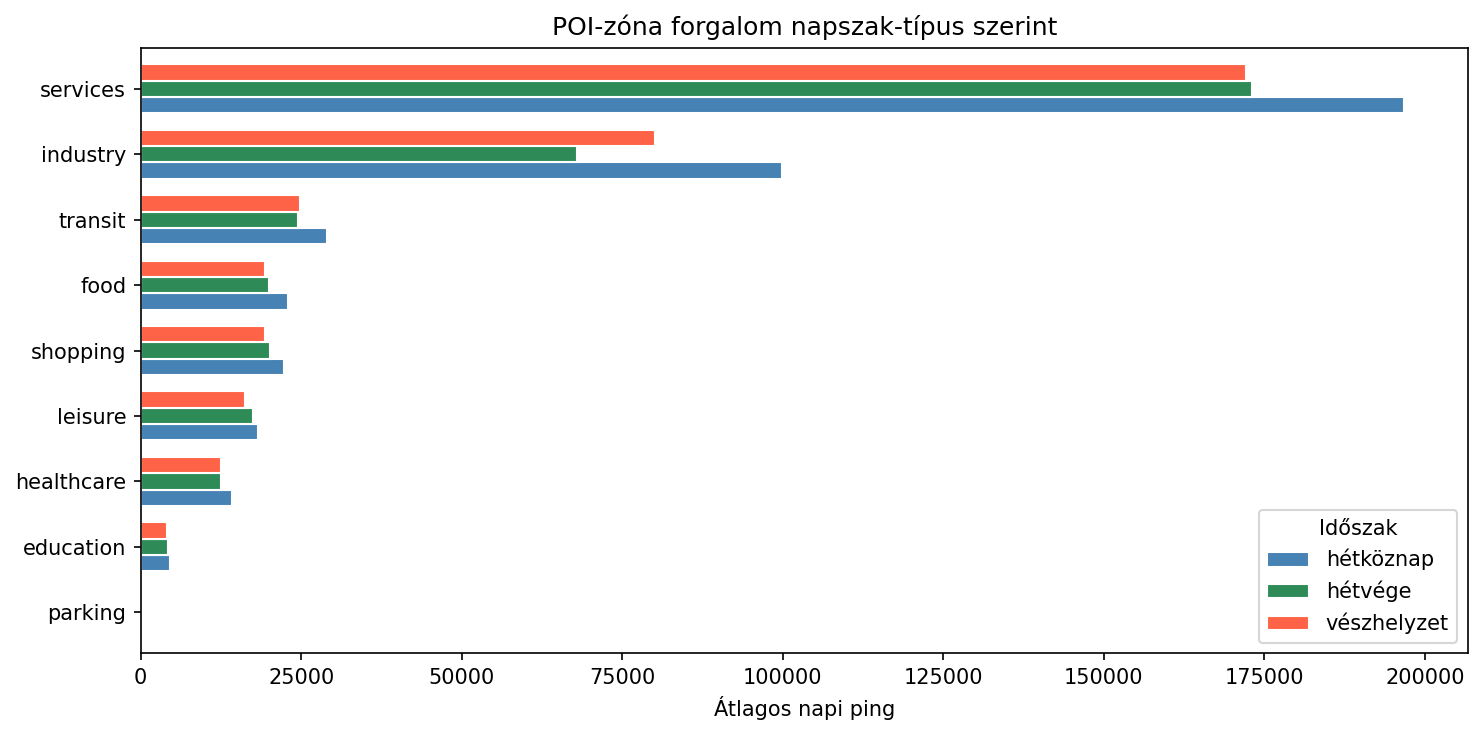
\includegraphics[width=0.90\textwidth]{img/impl_02_poi_by_period_type.png}
\caption{Aktivitás POI-zónák szerint, alap- és vészhelyzeti időszakban összehasonlítva. Saját számítás.}
\label{fig:impl02}
\end{figure}

\subsection{Anomáliadetekció eredményei}

\subsubsection{Napi anomáliaráta idősora}

A \autoref{fig:impl05} ábra a napi anomáliaráta idősorát ábrázolja a dataset2-n. Az alap-időszakban ($d < 60$) az anomáliaráta stabilan 7{,}0\% körül alakul. A vészhelyzeti időszakban ($d \geq 60$) a ráta 5{,}0\%-ra csökken.

\begin{figure}[H]
\centering
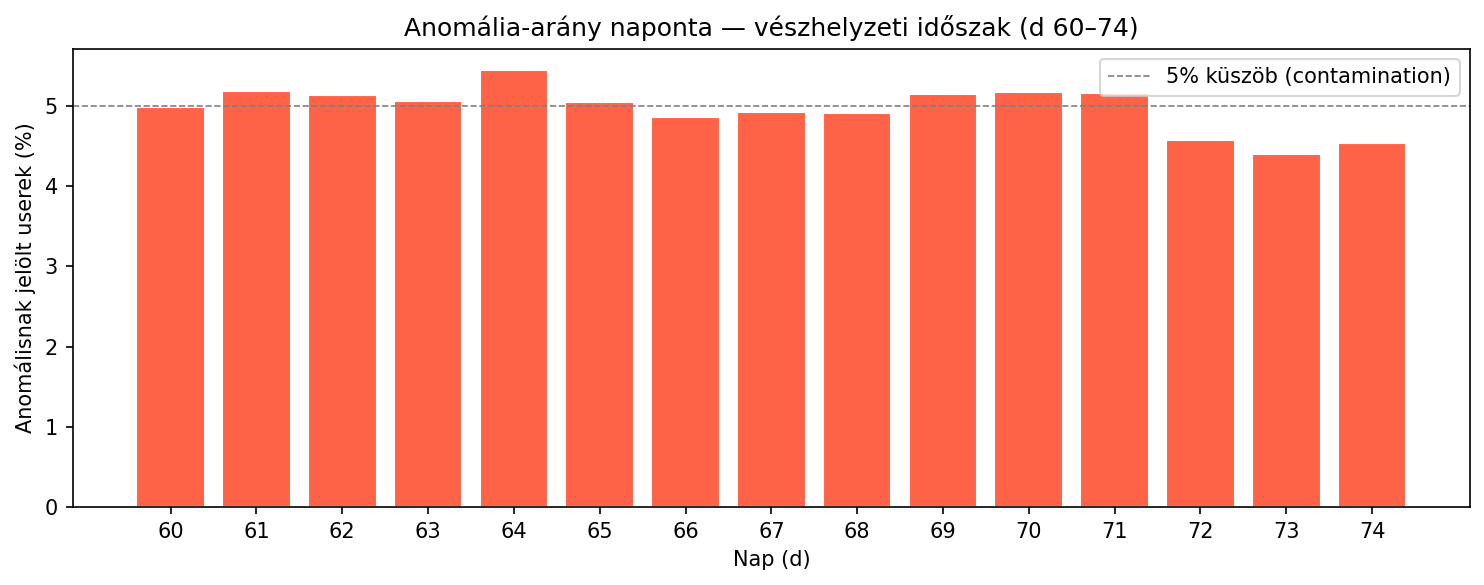
\includegraphics[width=0.90\textwidth]{img/impl_05_anomaly_daily_rate.png}
\caption{Napi anomáliaráta idősora a dataset2-n (alap- és vészhelyzeti szakasz). Saját számítás.}
\label{fig:impl05}
\end{figure}

Az eredmény látszólag ellentmondásos: a vészhelyzeti időszakban kevesebb anomáliát mértünk, holott éppen ekkor várnánk a rendellenes viselkedés arányának növekedését. A jelenség magyarázata, hogy a vészhelyzetben a mozgások kollektíven beszűkültek és egyöntetűbbé váltak, ezért az Isolation Forest --- amely a tipikus viselkedéstől való távolságot méri --- kevesebb mintát minősített szélsőségesnek. Aki mégis rendellenes maradt, az viszont annál kiugróbb értékeket mutatott, amint az a következő részben látszik.

\subsubsection{Anomális és normális felhasználók összehasonlítása}

A \autoref{fig:impl06} ábra a vészhelyzeti időszak anomális és normális felhasználóinak mobilitási jellemzőit veti össze boxplot-diagramokon. Az anomális felhasználók minden vizsgált dimenzióban szélsőséges értékeket mutatnak (\autoref{tab:anomaly_comparison}):

\begin{table}[H]
\centering
\caption{Anomális és normális felhasználók mobilitási jellemzőinek mediánjai a vészhelyzeti időszakban.}
\label{tab:anomaly_comparison}
\begin{tabular}{l r r r}
\hline
\textbf{Jellemző} & \textbf{Anomális} & \textbf{Normális} & \textbf{Arány} \\
\hline
Gyrációs sugár (m)         & 16~900 & 3~736  & 4{,}52× \\
Home--work távolság (m)    & 36~459 & 3~320  & 10{,}98× \\
Helydiverzitás (cella/nap) & 14     & 8      & 1{,}75× \\
\hline
\end{tabular}
\end{table}

\begin{figure}[H]
\centering
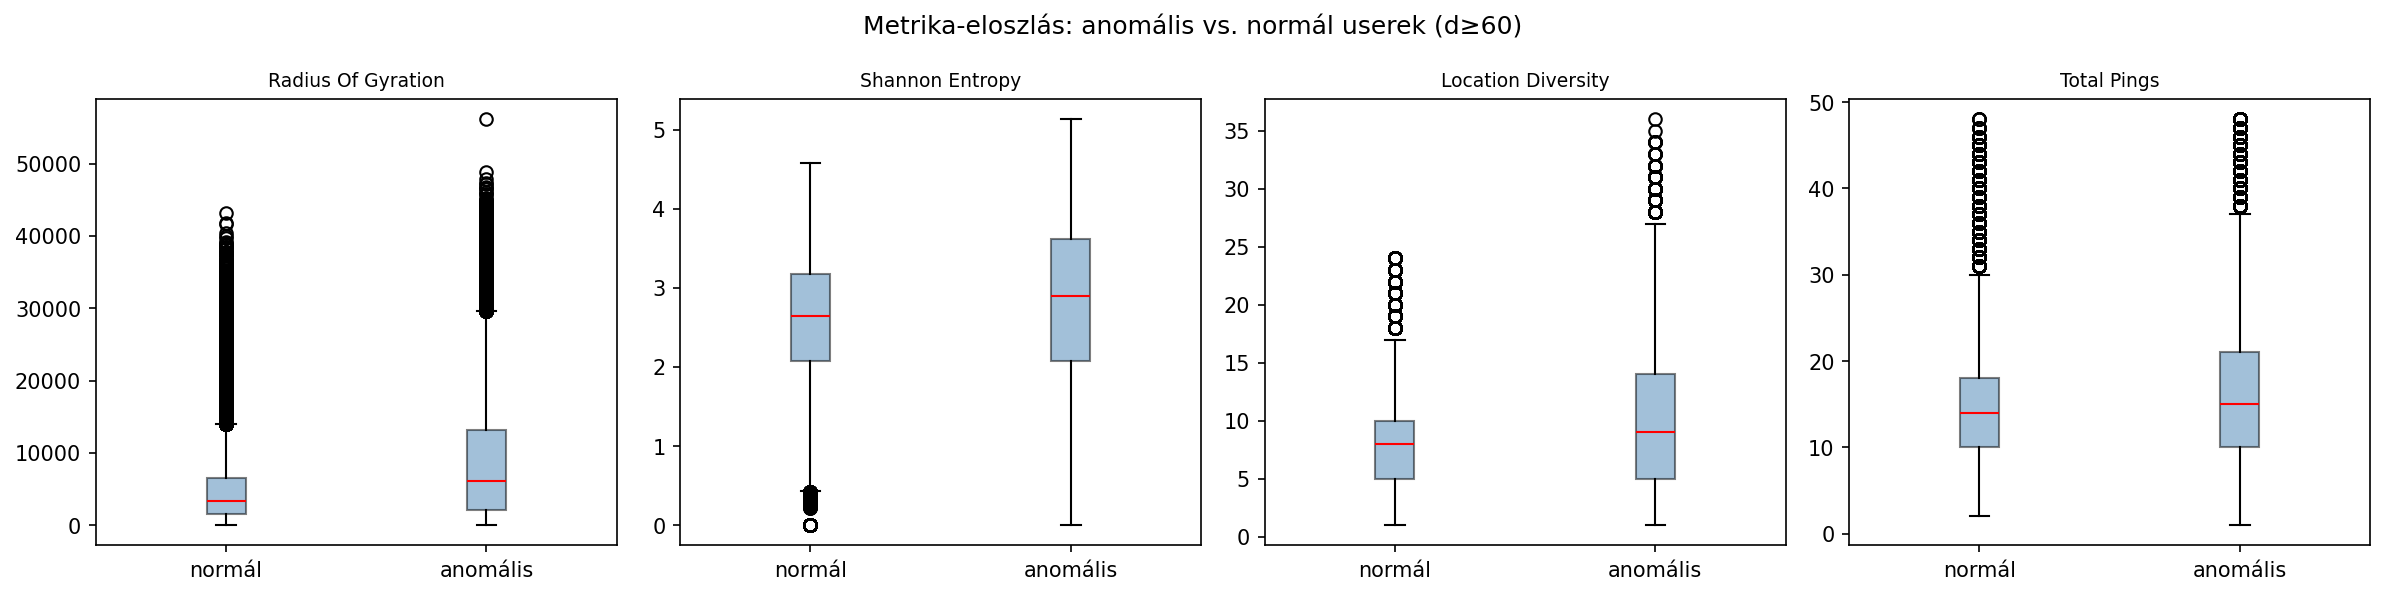
\includegraphics[width=0.90\textwidth]{img/impl_06_anomaly_feature_comparison.png}
\caption{Anomális és normális felhasználók jellemzőinek összehasonlítása boxplot-diagramokon, a vészhelyzeti időszakban. Saját számítás.}
\label{fig:impl06}
\end{figure}

A gyrációs sugár 4{,}52-szeres és a home--work távolság közel 11-szeres különbsége arra utal, hogy az anomális felhasználók lényegesen nagyobb területet jártak be a vészhelyzet alatt is --- vélhetően olyan egyének, akik nem tudtak otthon maradni, és hosszú, szokásostól eltérő útvonalakat tettek meg. Ez az eredmény összhangban áll Traag et al.\ \cite{traag2011social} esemény-detektálási megfigyeléseivel, miszerint rendkívüli helyzetekben a mobilhálózati adatban is mérhető szélsőséges mobilitás-növekedés figyelhető meg egy kisebb felhasználói csoportnál.

\subsection{Cirkadián ritmus és az "ébredő város" reprodukciója}
\label{subsec:circadian}

A Pintér és Felde \cite{pinter2022awakening} által Budapest mobilhálózati adatain bemutatott "ébredő város" jelenség --- vagyis a városi aktivitás reggeli felfutásának időzítése --- reprodukálható a YJMob100K adathalmazon is. A \autoref{fig:circ01} ábra a 30~perces időrésekre aggregált átlagos aktivitást ábrázolja a normál (dataset1) és a vészhelyzeti (dataset2, $d \geq 60$) időszakra.

\begin{figure}[H]
\centering
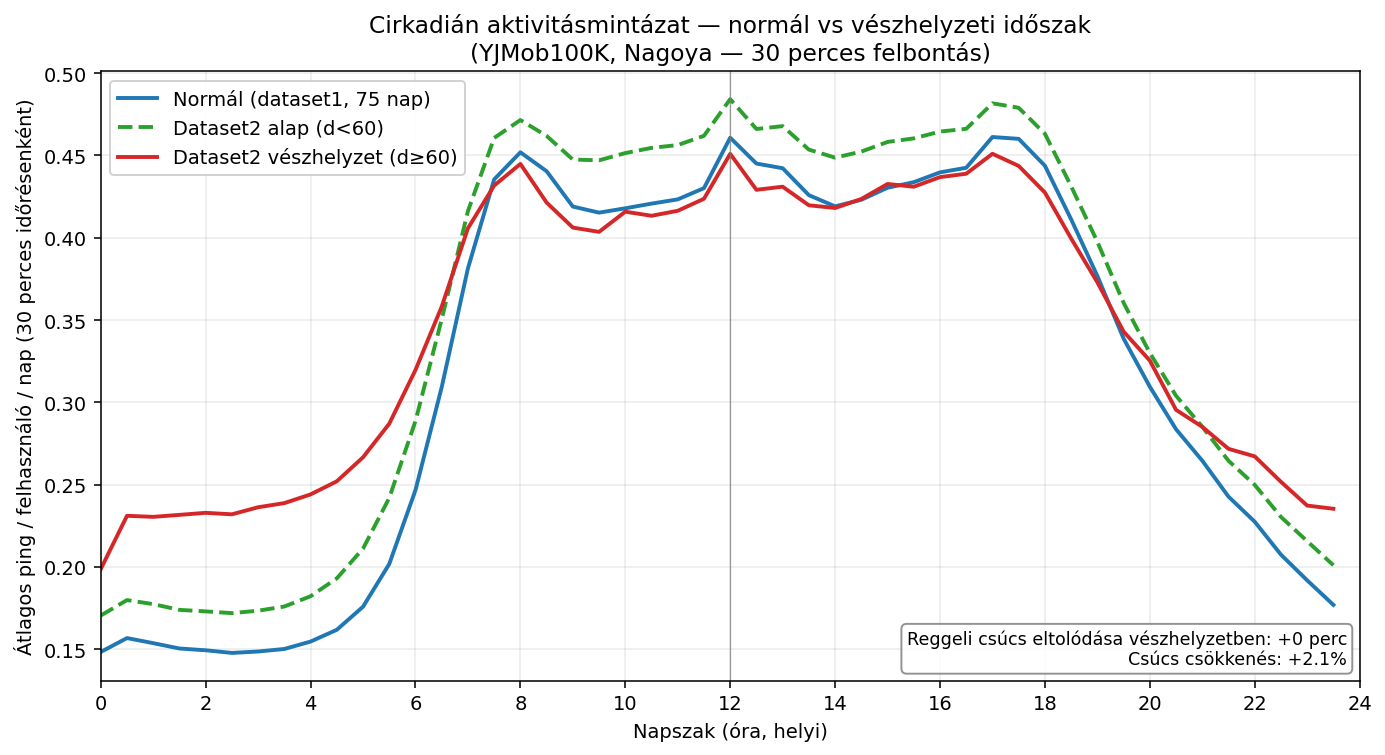
\includegraphics[width=0.95\textwidth]{img/circ_01_circadian_comparison.png}
\caption{Aggregált napi aktivitás-görbe normál és vészhelyzeti időszakra. Saját számítás.}
\label{fig:circ01}
\end{figure}

Az "ébredési idő" formálisan az a $t_{\mathrm{wake}}$ időpont, amelynél az aggregált aktivitás felfelé tartva eléri az éjszakai alapérték és a nappali plató közötti 50\,\%-os küszöböt (Pintér és Felde \cite{pinter2022awakening} módszertanát követve, lineáris interpolációval a két szomszédos időrés között). Ezzel a definícióval $t_{\mathrm{wake}}$ a normál időszakban 6{,}38~óra (kb.\ 06:23), a vészhelyzet előtti dataset2 alapidőszakban 6{,}25~óra, a vészhelyzet alatt pedig 6{,}14~óra (kb.\ 06:08). A vészhelyzet tehát mintegy 9--14~perccel előrébb tolta a kollektív ébredést, miközben az éjszakai (00:00--05:00) aktivitás 53{,}0\%-kal nőtt, a nappali plató szintje viszont csak 1{,}8\%-kal csökkent. Ez az aszimmetria jól illeszkedik Pintér és Felde \cite{pinter2022awakening} azon megfigyeléséhez, hogy a rendkívüli helyzetek nem feltétlenül a teljes aktivitást, hanem inkább annak időzítését és összetételét változtatják meg.

\subsection{Felhasználói archetípusok K-Means klaszterezéssel}
\label{subsec:archetypes}

A Pintér \cite{pinter2020artificial} disszertációjában leírt mobilitási archetípusok reprodukálhatók a YJMob100K adatokon is. Mind a 100~000 dataset1-beli felhasználóra K-Means algoritmust ($k=4$, \texttt{random\_state}=42) futtattunk három log-transzformált és skálázott napi metrikán: gyrációs sugár, Shannon-entrópia és otthon--munkahely távolság.

\begin{figure}[H]
\centering
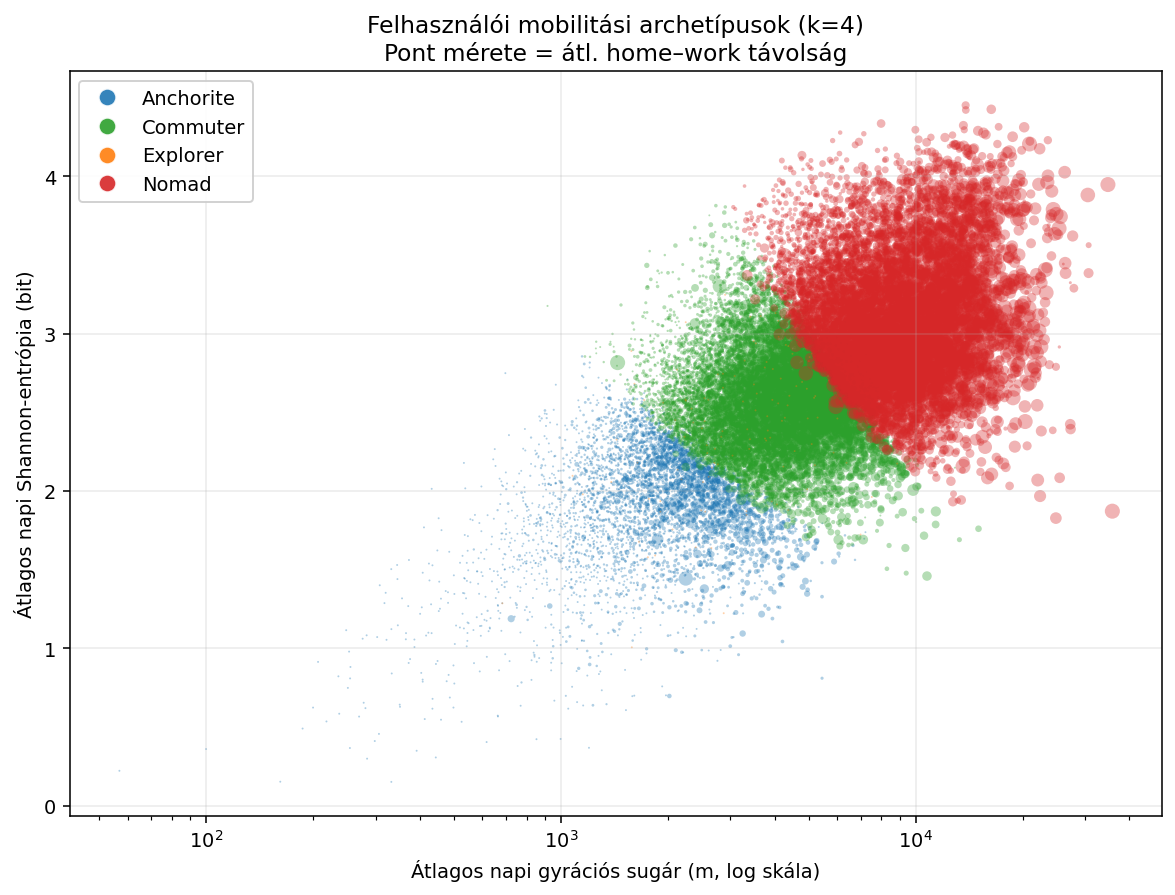
\includegraphics[width=0.95\textwidth]{img/seg_01_cluster_scatter.png}
\caption{A négy klaszter elhelyezkedése a (gyrációs sugár, home--work távolság) síkon. Saját számítás.}
\label{fig:seg01}
\end{figure}

A \autoref{tab:archetypes} foglalja össze a kapott három érdemi klaszter jellemzőit. A negyedik klaszter (4{,}2\%, NULL munkahely-cellával) inkább adatminőségi (mintavételezési) műtermek, mint valódi viselkedési típus. A három érdemi archetípus interpretációja:
\begin{itemize}
\item \textbf{Anchorite} (15{,}3\%) --- alacsony gyrációs sugar ($\approx$1{,}86~km), kis home--work távolság, valószínűleg helyhez kötött nyugdíjasok vagy otthon dolgozók.
\item \textbf{Commuter} (45{,}0\%) --- közepes gyrációs sugar ($\approx$3{,}89~km), tipikus 5{,}5~km-es home--work távolsággal: a klasszikus városi ingázók.
\item \textbf{Nomad} (35{,}5\%) --- magas gyrációs sugar ($\approx$8{,}17~km) és nagy home--work távolság ($\approx$14{,}40~km): nagy területet bejáró felhasználók (távingázók, sokat utazók).
\end{itemize}

\begin{table}[H]
\centering
\caption{A K-Means klaszterezés eredményei (dataset1, $k=4$, $n=100\,000$ felhasználó). Mediánok, a \texttt{10-user-segments.ipynb} újrafuttatásából.}
\label{tab:archetypes}
\begin{tabular}{l r r r r r}
\hline
\textbf{Archetípus} & \textbf{N} & \textbf{Részarány} & \textbf{R\textsubscript{g} (m)} & \textbf{H--W (m)} & \textbf{Diverzitás (cella/nap)} \\
\hline
Anchorite & 15\,332 & 15{,}3\% &  1\,855 &  1\,861 &  5{,}7 \\
Commuter  & 45\,025 & 45{,}0\% &  3\,887 &  5\,464 &  7{,}8 \\
Nomad     & 35\,450 & 35{,}5\% &  8\,173 & 14\,395 & 10{,}5 \\
\hline
\end{tabular}
\end{table}

A klaszterek térbeli megoszlását a \autoref{fig:seg02} ábra szemlélteti Nagoya OpenStreetMap alaptérképén: a Nomad-felhasználók a peremkerületekben és vasútvonalak mentén, az Anchorite-ok pedig a sűrűbben lakott belvárosban koncentrálódnak --- ez a térbeli mintázat összhangban van Pintér és Felde \cite{pinter2021evaluating} szocioökonómiai gradiensről szóló eredményével.

\begin{figure}[H]
\centering
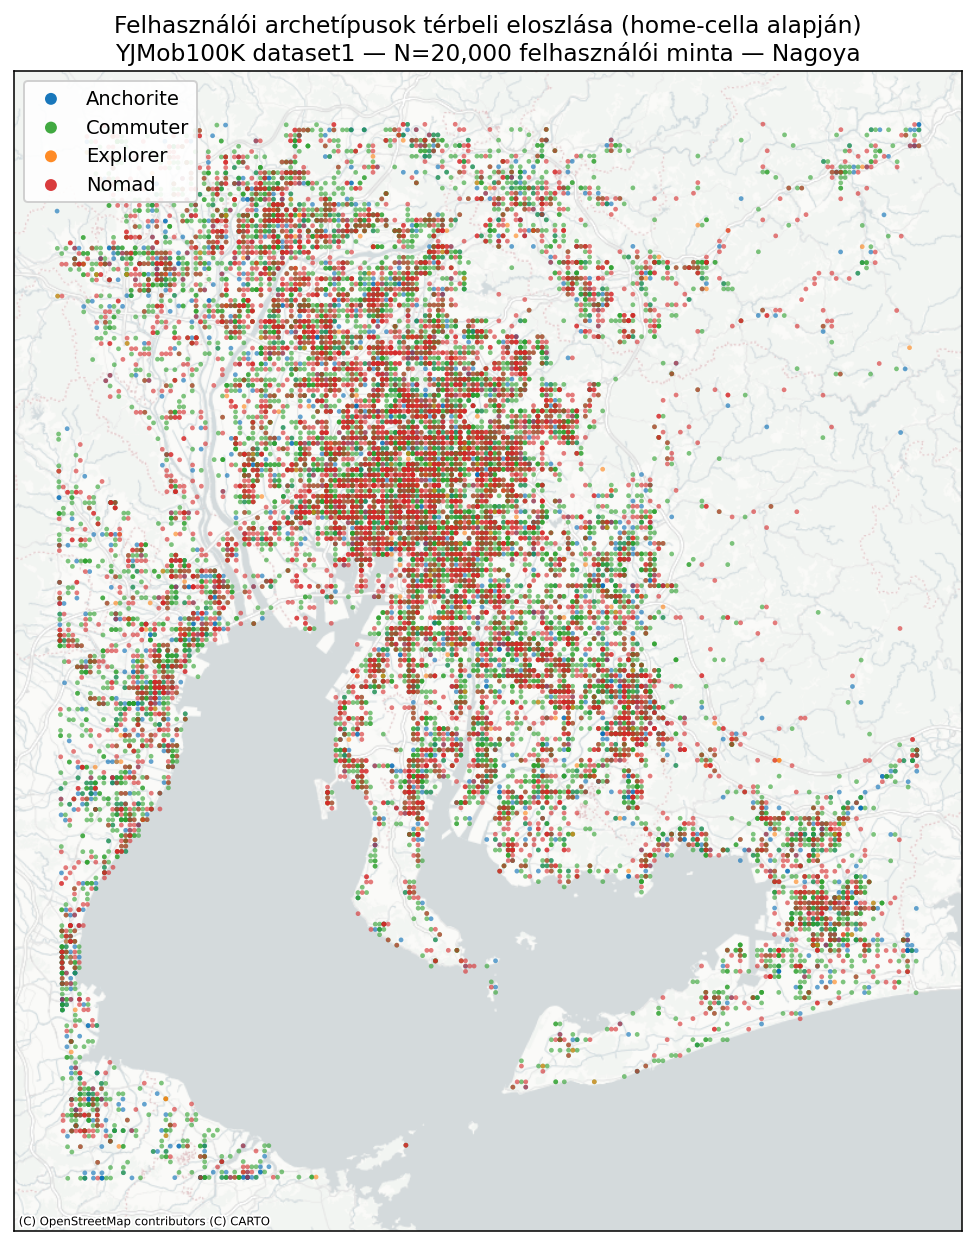
\includegraphics[width=0.95\textwidth]{img/seg_02_cluster_gis.png}
\caption{Az archetípusok otthonainak térbeli eloszlása Nagoya OSM-térképen. Saját számítás.}
\label{fig:seg02}
\end{figure}


